\documentclass[a4paper]{article}
\usepackage[utf8]{inputenc}
\usepackage[russian,english]{babel}
\usepackage[T2A]{fontenc}
\usepackage[left=10mm, top=20mm, right=18mm, bottom=15mm, footskip=10mm]{geometry}
\usepackage{indentfirst}
\usepackage{amsmath,amssymb}
\usepackage[italicdiff]{physics}
\usepackage{graphicx}
\graphicspath{{images/}}
\DeclareGraphicsExtensions{.pdf,.png,.jpg}
\usepackage{wrapfig}

\usepackage{caption}
\captionsetup[figure]{name=Рисунок}
\captionsetup[table]{name=Таблица}

\title{\underline{Отчет о выполненой лабораторной работе 1.3.1}}
\author{Воронин Денис, Б04-403}

\begin{document}

\maketitle
\begin{center}
    \textbf{Определение модуля Юнга на основе
    исследования деформаций растяжения}
\end{center}

\section{Аннотация}
\textbf{Цель работы:} экспериментально получить зависимость между напряжением и деформацией
(закон Гука) для простейших напряженных состояний упругих тел одноосного растяжения.
деформацией

\textbf{В работе используются:}прибор Лермантова, проволока из исследуемого материала, зрительная
труба со шкалой, набор грузов, микрометр, 2-х метровая линейка.

\section{Теоретические сведения}
Связь между удлинением проволоки $\bigtriangleup l$ и силой Р, вызывающей это удлинение, выражается
законом Гука:\par
\[\frac{P}{S} = E\frac{\bigtriangleup l}{l}\]  
где l - начальная длина проволоки,S - ее сечение, Е - константа, характеризующая упругие
свойства материала (модуль Юнга).

\section{Устройство прибора}
\begin{wrapfigure}{l}{0.5\textwidth}
    \centering
    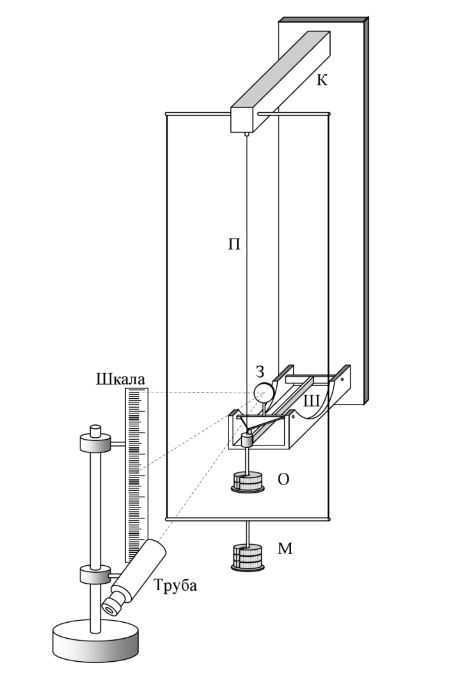
\includegraphics[width=0.4\textwidth]{pick1.PNG}
\end{wrapfigure}
Для определения модуля Юнга в этой работе используется прибор Лермантова, схема
которого изображена на рис. 1. Верхний
конец проволоки $\textbf{\text{П}}$, изготовленный
исследуемого материала, прикреплён
кронштейну $\textbf{\text{К}}$, а нижний к цилиндру, которым
оканчивается шарнирный
кронштейн $\textbf{\text{Ш}}$.На этот же цилиндр
опирается рычаг $\textbf{\text{r}}$, связанный с зеркальцем
$\textbf{\text{З}}$. Таким образом, удлинение проволоки
Можно измерить по углу поворота
зеркальца. \par
Натяжение проволоки можно менять,
перекладывая груз C площадки $\textbf{\text{М}}$ на
площадку $\textbf{\text{О}}$ и наоборот. Такая система
позволяет исключить влияние деформации
кронштейна $\textbf{\text{К}}$ на точность измерений, т. к.
нагрузка на нём все время остается 
постоянной.\par
При проведении эксперимента
следует иметь в виду, что проволока $\textbf{\text{П}}$ при
отсутствии нагрузки всегда несколько
изогнута, что не может не сказаться на
результатах, особенно при небольших
нагрузках. Выпрямить проволоку путём
увеличения начальной нагрузки опасно, т. к.
при этом можно выйти за границу
применимости закона Гука (возникнут
остаточные деформации).
\newpage

\section{Ход работы}
\subsection{Составление таблицы}

\begin{table}[!h]
    \begin{center}
    \begin{tabular}{|l|l|l|l|l|l|l|l|l|}
    \hline
    & $m$, гр & $P$, Н & $n_1 \downarrow$, см & $n_1\uparrow$, см &$\bigtriangleup \overline{n} $ &$\bigtriangleup \overline{l} $  \\ \hline
    1                       & 0,724&        7,24&      23,0&   23,0 &   0&   0        \\ \hline
    2                       & 0,970&        9,70&      24,2&   24,2&   1,2&   3,2       \\ \hline
    3                        & 1,215&       12,15&     25,0&   25,9&   1,25&  4,45   \\ \hline
    4                        & 1,460&       14,60&     26,8&   26,9&   1,4&   5,85        \\ \hline
    5                        & 1.705&       17,05&     28,0&   28,2&   1,25&  7,1     \\ \hline
    6                        & 1,950&       19,50&     29,1&   29,4&   1,15&  8,25         \\ \hline
    7                        & 2,196&       21,96&     30,3&   30,9&   1,35&  9,6        \\ \hline
    8                        & 2,441&       24,41&     31,6&   31,4&   0,9&   10,5     \\ \hline
    9                        & 2,686&       26,86&     32,7&   32,5&   1,1&   11,6      \\ \hline
    10                        & 2,931&      29.31&     33,9&   33,9&   1,3&   12,9     \\ \hline

    \end{tabular}
    \caption{Зависимость покааний шкалы от нагрузки}
    \end{center}
    \end{table}

\begin{table}[!h]
    \begin{center}
    \begin{tabular}{|l|l|l|}
    \hline
        $d$, мм&  $h$, см& $l$, см \\ \hline
        0,26$\pm $ 0,01& 149$\pm $0,1&176,5$\pm $0,1  \\ \hline
    \end{tabular}
    \caption{Параметры установки}
    \end{center}
\end{table}


1.Найдем площадь поперечного сечения проволоки:
\[S = \frac{\pi (\overline{d})^2}{4} = 0,053 \text{мм}^2 \]
\[\sigma_{s} = S\sqrt{2(\frac{\sigma_{s}}{d})^2 } = 0,003 \text{мм}^2\]
\[S = (0,053\pm 0,003) \text{мм}^2\]
2.Направляем зрительную трубу на зеркальце так, чтобы мы четко видели шкалу, тогда свет от шкалы будет падать примерно перпендикулярно шкале на зеркало, поэтому удлинение проволоки можно выразить так:
\[\Delta l =\dfrac{nr}{2h}\]
\[ \sigma_{\Delta l} = \Delta l\sqrt{\left( \dfrac{\sigma_{n}}{n}\right)^2 + \left(\dfrac{\sigma_d}{d}\right)^2+\left(\dfrac{\sigma_h}{h}\right)^2} \]
где $r = 20\pm 0,1$ см - длина рычага, разница показаний шкалы - $n$, расстояние от шкалы до проволоки - $h = (149\pm0,1)\text{ см}$.\par
3.Исходя из того, что $\sigma_{\text{предел}} = 900 \text{ Н}/\text{мм}^2$ получаем, что предельный вес, который можно повесить, чтобы не выйти за пределы $P_{\text{предел}} = 0,3 \sigma_{\text{предел}} S \approx 44,8 H$.\par
4.Снимем зависимость удлинения проволоки от массы грузов при увеличении и уменьшении нагрузки  (табл.1). \par
5.Построим график зависимости удлинения проволоки от нагрузки. В недеформированном состоянии проволока, как правило, изогнута, и при малых нагрузках её "удлинение" определяется не растяжением, а выпрямлением. Найдем уравнение получившийся прямой по МНК. По наклону прямой определим жесткость проволоки, а по ней - модуль Юнга (табл.2). Начальный участок графика при обработке следует исключить.\par
6.Используя программу на Python данные из таблицы 1 вычислим уравнение наилучшей прямой для графика в координатах $m_{(\bigtriangleup l )}$:\par

\[m = 0.182\bigtriangleup l + 0.492\]
\[\sigma_k = k\sqrt{(\frac{\sigma_\bigtriangleup m}{\bigtriangleup m} )^2 + (\frac{\sigma \bigtriangleup l}{\bigtriangleup l} )^2}\] 
Откуда $k = 1.82\pm 0.12 $ кг/м\par

7. Определим модуль Юнга и его погрешность по формулам 
\[E = k\frac{lg}{S}\]
\[\sigma_E = \sqrt{\left( \dfrac{\sigma_{k}}{k} \right)^2 + \left( \dfrac{\sigma_{S}}{S} \right)^2 + \left( \dfrac{\sigma_{l_0}}{l_0} \right)^2 }\]
\begin{flushleft}
$\sigma_E = 0.1 \text{ГПа}$\par
$E = 120.3$ ГПа\par
8. Сравнивая полученное значение модуля Юнга с табличным, можно увидеть, что данное значение соответсвует меди (110-125 ГПа)
\end{flushleft}

\begin{figure}[h]
    \centering
    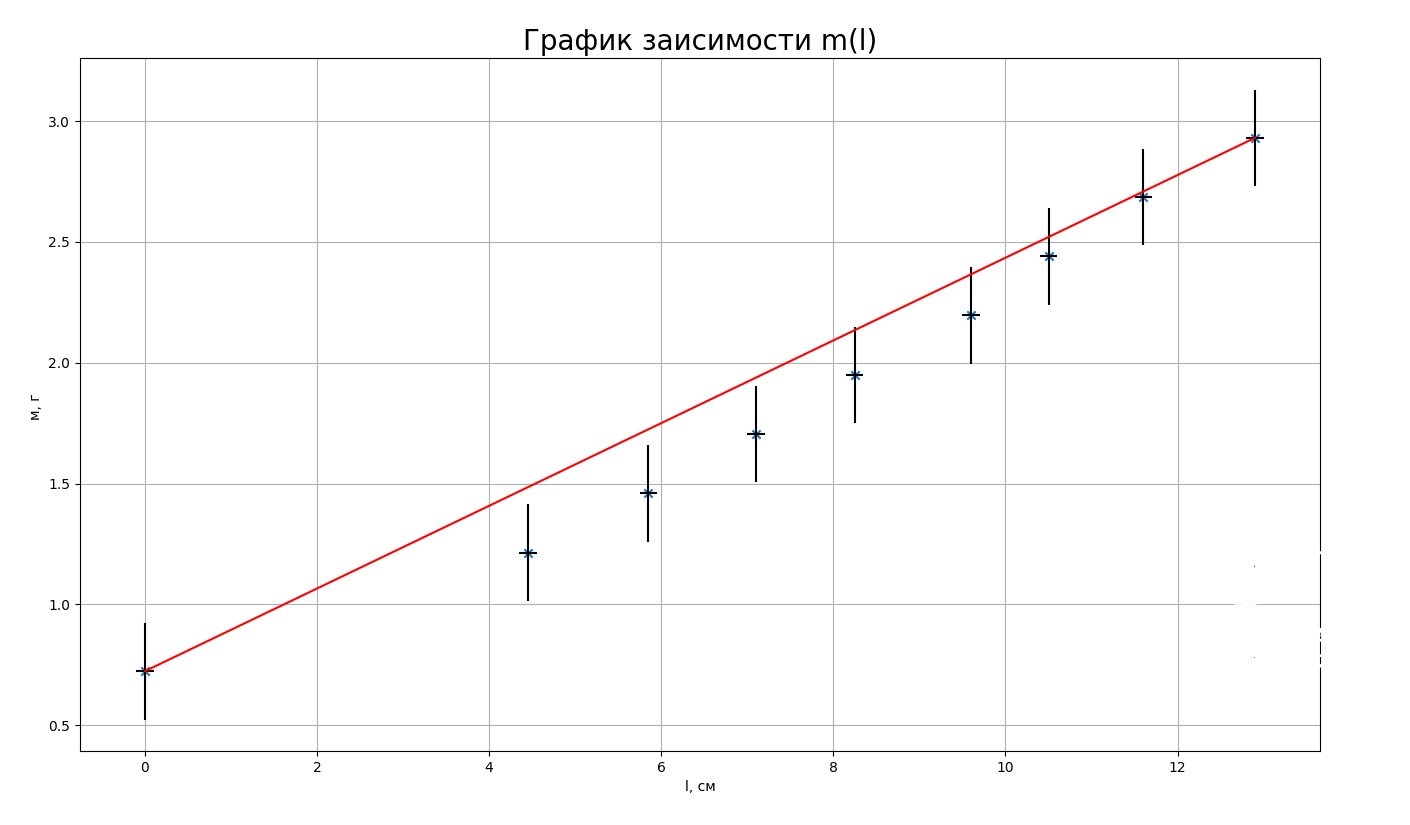
\includegraphics[width=1\textwidth]{pick2.PNG} 
    \caption{График $m\bigtriangleup l$}
    \end{figure}




\end{document}